\newcommand{\prompt}[1]{\lstinline[style=promptstyle]!#1!}

\section{Qwen3-ASR}

\subsection{Architecture}

\begin{figure}[h]
    \centering
    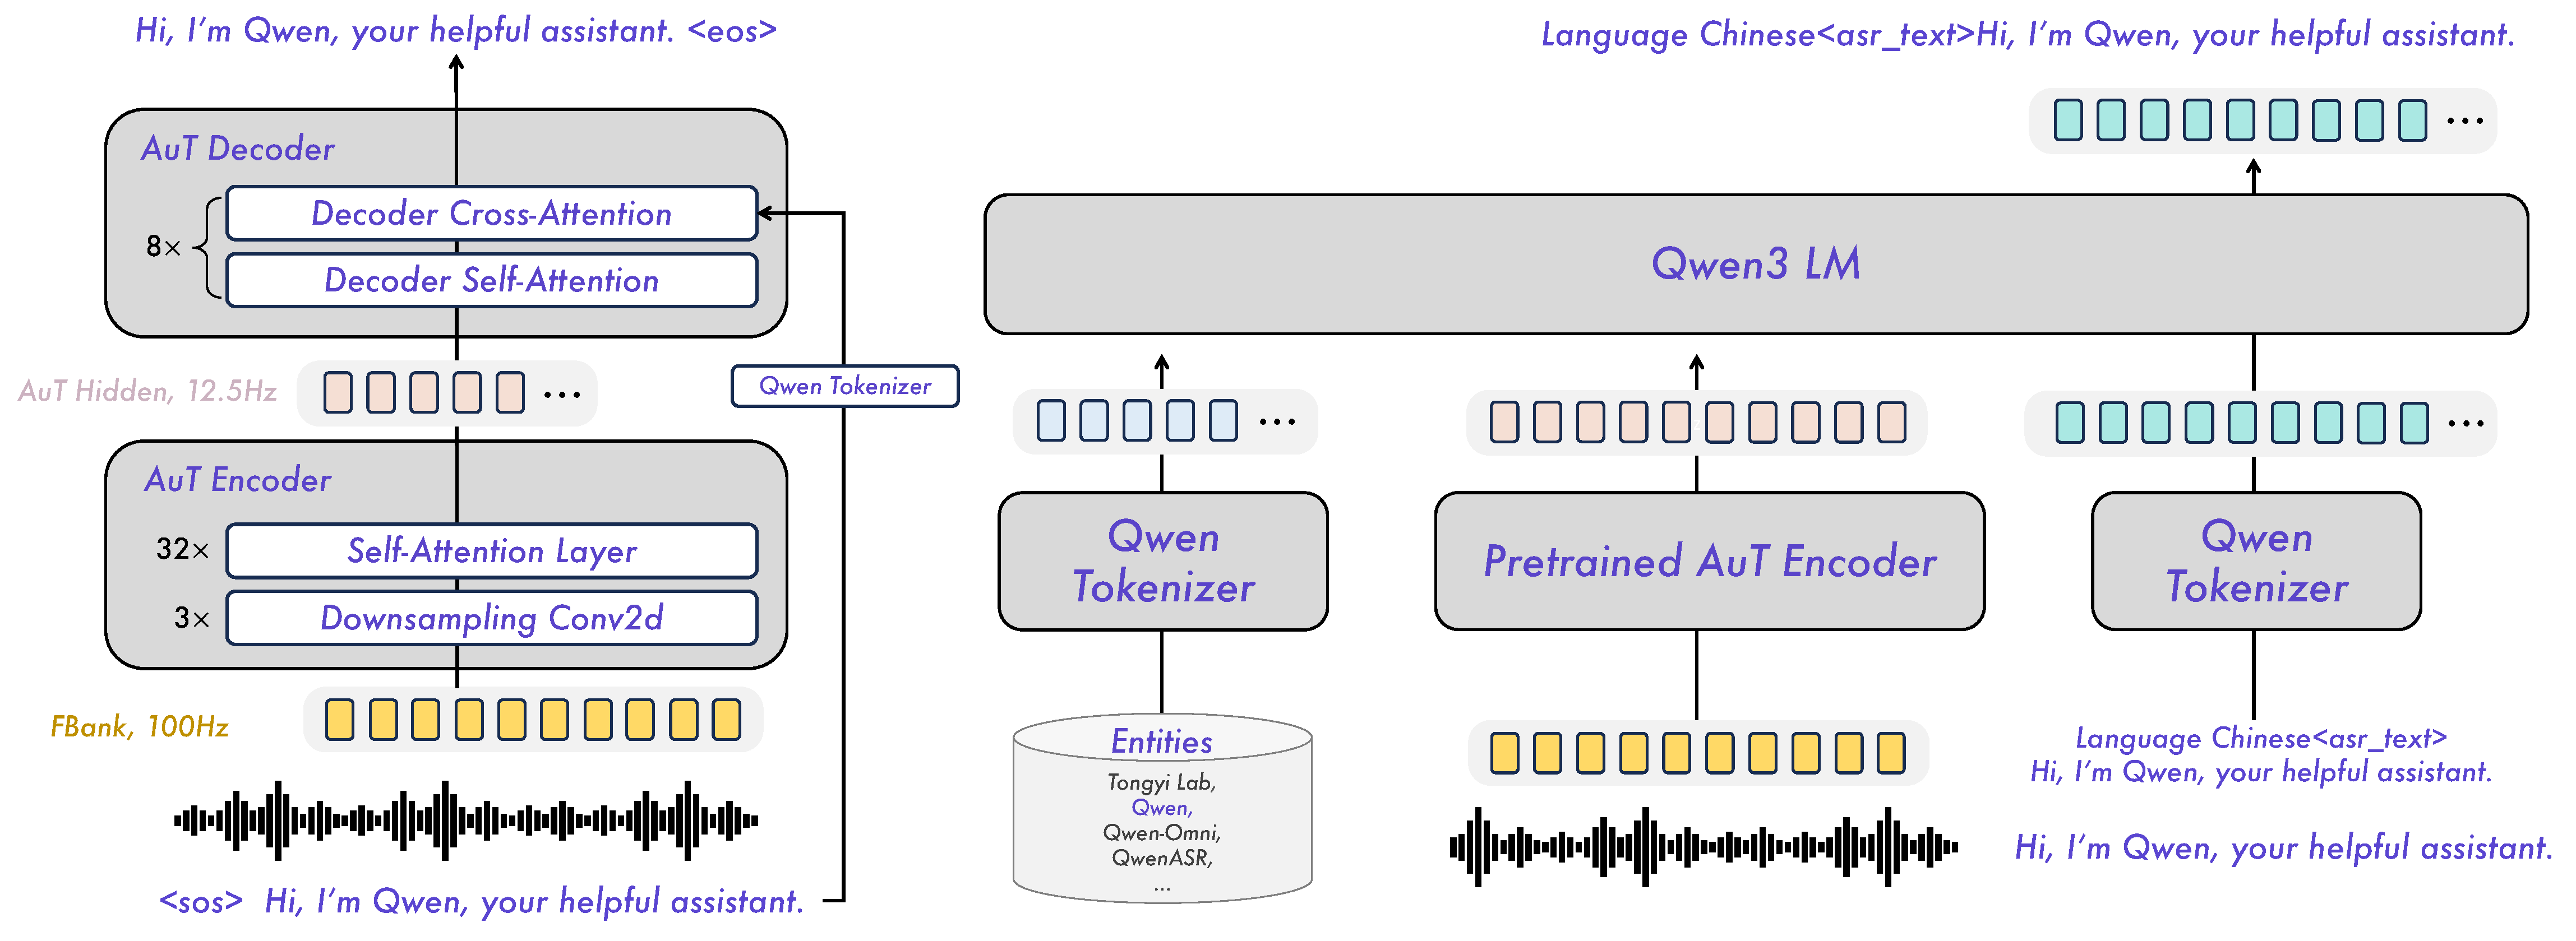
\includegraphics[width=1.0\linewidth]{figures/overview.pdf}
    \caption{Architecture of AuT~(left) and the overview of Qwen3-ASR~(right).}
    \label{fig:aut}
\end{figure}

Qwen3-ASR family models leverage Qwen3-Omni as a foundation model, which proved to obtain strong audio understanding ability~\citep{arxiv2025-jinxu-qwen3omni}. Speech to recognize is first fed to AuT encoder, which is pretrained separately from Qwen3-Omni and Qwen3-ASR. As illustrated in Figure~\ref{fig:aut}(left), AuT is an attention-encoder-decoder~(AED) based ASR model which conducts 8 times downsampling to Fbank feature with 128 dimensions, yielding a 12.5Hz token rate audio encoder. We use a dynamic flash attention window size ranging from 1s to 8s, which allows Qwen3-ASR to perform both streaming inference with short chunks and offline inference with long queries. The architecture of models we are releasing is illustrated as Figure~\ref{fig:aut}(right) and detailed as below: \textbf{Qwen3-ASR-1.7B} is built with Qwen3-1.7B, a projector, and an AuT encoder with 300M parameters and 1024 hidden size. This model demonstrates strong performance in multilingual and dialect speech recognition, so as well as robustness under complex acoustic environment and text patterns. \textbf{Qwen3-ASR-0.6B} is built with Qwen3-0.6B, a projector and an AuT encoder with 180M parameters and a hidden size of 896. We design this compact model to balance recognition accuracy and inference efficiency, while remaining highly competitive among sub-1B-parameter ASR models.

% \begin{itemize}
%     \item \textbf{Qwen3-ASR-0.6B} is built with Qwen3-0.6B, a projector and an AuT encoder with 180M parameters and 896 hidden size.
%     \item \textbf{Qwen3-ASR-1.7B} is built with Qwen3-1.7B, a projector and the AuT encoder has 300M parameters and 1024 hidden size.
% \end{itemize}

% Qwen3-ASR series models are composed of an audio encoder, a projector and Qwen LLM. The audio encoder is pretrained in audio Transformer~(AuT), an attention-encoder-decoder model as illustrated in Fig~\ref{fig:aut}~(a). The encoder of AuT conducts 8 times downsampling over fbank features with Conv2d blocks, reducing the token rate to 12.5Hz. The attention layers then extract hidden representation with dynamic flash attention covering attention query patterns ranging from 1s to 8s. AuT encoder thus obtained balanced inference performance of both offline and streaming ASR.
% Beyond unified streaming/non-streaming inference, the Qwen3-ASR family features the following highlights:
% \begin{itemize}
% \item \textbf{Unified streaming/non-streaming inference.} 
% \item \textbf{Free-form contextual biasing.} Qwen3-ASR is trained to accept free-form text at the beginning of the prompt as contextual information or background knowledge, enabling users to obtain customized recognition results with an entity list, a paragraph, or even unstructured text.
% \item \textbf{Language Identification.} Qwen3-ASR reliably identifies the spoken language before performing speech recognition.
% \end{itemize}

\subsection{Training Strategies}
\label{section:traning-strategies}

The training process of Qwen3-ASR consists of AuT pretraining, Omni pretraining, and ASR post-training, where the first two stages are identical to those of Qwen3-Omni.
\begin{enumerate}[label=(\arabic*)]
    \item \textbf{AuT pretraining.} In this stage, we aim to obtain a pretrained encoder under the AED framework using large-scale labeled data. We leverage approximately 40 million hours of pseudo-labeled ASR data, where the majority is in Chinese and English. This pretrained encoder is shown to provide general and stable audio representations under dynamic attention window sizes.

    \item \textbf{Omni pretraining.} We use the pretrained Qwen3-Omni model as the foundation model for ASR training. Omni pretraining is conducted on multi-task audio, vision, and text data. In this stage, both Qwen3-ASR-0.6B and Qwen3-ASR-1.7B are trained with 3 trillion tokens, acquiring multi-modal understanding capability. The detailed training pipeline follows \citep{arxiv2025-jinxu-qwen3omni}.

    \item \textbf{ASR supervised finetuning (SFT).} In the SFT stage, we perform style transfer on the ASR input/output format with a substantially smaller set of multilingual data that is disjoint from the pretraining corpus. Besides standard Chinese, English and multilingual ASR data, SFT stage also utilizes non-speech data, streaming-enhancement data and context biasing data. Specifically, we train the model to be an ASR-only model that does not follow natural-language instructions in the prompt, in order to mitigate instruction injection and instruction-following failures. The output of Qwen3-ASR has outputs in two types for the given audio, with and without recognizable human speech:

    \definecolor{chatmlblue}{RGB}{0, 0, 255}
    % gbsn
    \begin{CJK*}{UTF8}{gkai}
    \resizebox{0.925\textwidth}{!}{%
    \begin{tcolorbox}[
        % Box styling
        colback=lightgray,
        colframe=black,
        boxrule=1pt,
        %sharp corners,
        width=\textwidth,
        % Title styling
        title={Qwen3-ASR output style},
        colbacktitle=black,
        coltitle=white,
        fonttitle=\bfseries\sffamily,
        halign title=left,
        % halign=left
    ]
    % Use a monospaced font for the content
    % \ttfamily
    % First user-assistant exchange
    \textbf{Output style 1: For recognizable speech}\\
    \textbf{<|im\_start|>}assistant \\
    language English\textbf{<asr\_text>}Today we release models including Qwen3-ASR-1.7B.\textbf{<|im\_end|>} \\
    %\textbf{<|im\_start|>}assistant \\
    %language Chinese\textbf{<asr\_text>}今天我们发布包括Qwen3-ASR-1.7B在内的模型。\textbf{<|im\_end|>} \\
    
    \textbf{Output style 2: For no speech detected}\\
    \textbf{<|im\_start|>}assistant \\
    language None\textbf{<asr\_text><|im\_end|>}
    \end{tcolorbox}
    }
    \end{CJK*}
    Meanwhile, the model learns to utilize the context tokens inside the system prompt as background knowledge, allowing users to obtain customized ASR results.
    
    % \begin{CJK*}{UTF8}{gkai}
    % \resizebox{0.925\textwidth}{!}{%
    % \begin{tcolorbox}[
    %     % Box styling
    %     colback=lightgray,
    %     colframe=black,
    %     boxrule=1pt,
    %     %sharp corners,
    %     width=\textwidth,
    %     % Title styling
    %     title={Qwen3-ASR contextual biasing style},
    %     colbacktitle=black,
    %     coltitle=white,
    %     fonttitle=\bfseries\sffamily,
    %     halign title=left,
    %     % halign=left
    % ]
    % \textbf{Context style 1: Words list}\\
    % \textbf{<|im\_start|>}system \\
    % 通义千问, Qwen3-max, Qwen3-ASR-1.7B, Qwen3-Image-Edit ...\textbf{<|im\_end|>} \\

    % \textbf{Context style 2: Freeform text}\\
    % \textbf{<|im\_start|>}system \\
    % Qwen recently released VL model Qwen3-VL and Qwen3-Image-Edit, audio model Qwen3-TTS and Qwen3-ASR-1.7B and a lot of models on the way.\textbf{<|im\_end|>} \\
    
    % ... (other freeform or even unorganized text as context)
    % \end{tcolorbox}
    % }
    % \end{CJK*}

    \item \textbf{ASR reinforcement learning (RL).} At the last stage, we use Group Sequence Policy Optimization~(GSPO, ~\cite{zheng2025group}) for further improving the quality of recognition. It turns out that RL plays an essential role in models' noise robustness, transcription stability and ability to analyze difficult cases. The total data leveraged by RL stage is about 50k utterances including 35\% Chinese and English data, 35\% multilingual data and 30\% functional data, which aims at improving transcribing stability in complex environments.
\end{enumerate}

\subsection{Features}
\label{method:features}

With the architecture and training strategies introduced above, Qwen3-ASR family models are notable in the aspects below:

\begin{table}[ht]
\centering
\caption{\textbf{Features of the Qwen3-ASR model family. Qwen3-ASR-1.7B and Qwen3-ASR-0.6B support 52 languages and dialects, comprising 30 languages and 22 Chinese dialects. Qwen3-ForcedAligner-0.6B supports 11 languages. Seq. Len. denotes the maximum audio length for single inference in seconds, and NAR denotes non-autoregressive inference.}}
\label{tab:feature-new}
\renewcommand{\arraystretch}{1.15}
\setlength{\tabcolsep}{2.5pt}
\footnotesize

\resizebox{\textwidth}{!}{%
\begin{tabular}{
>{\centering\arraybackslash}m{3.2cm}
>{\raggedright\arraybackslash}m{4.8cm}
>{\raggedright\arraybackslash}m{5.4cm}
>{\centering\arraybackslash}m{2.2cm}
>{\centering\arraybackslash}m{1.8cm}
>{\centering\arraybackslash}m{2.8cm}
}
\toprule
\multirow{2}{3.2cm}{\centering \textbf{Model}} & \multirow{2}{4.8cm}{\raggedright \textbf{Supported Languages}} & \multirow{2}{5.4cm}{\raggedright \textbf{Supported Dialects}} & \multirow{2}{2.2cm}{\centering \textbf{Inference Mode}} & \multirow{2}{1.8cm}{\centering \textbf{Seq. Len.}} & \multirow{2}{2.8cm}{\centering \textbf{Audio Types}} \\
& & & & & \\
\midrule

\multirow{8}{3.2cm}{\centering \textbf{Qwen3-ASR-1.7B} \&\\ \textbf{Qwen3-ASR-0.6B}}
&
\makecell[l]{Chinese (zh), English (en),\\
Cantonese (yue), Arabic (ar),\\
German (de), French (fr),\\
Spanish (es), Portuguese (pt),\\
Indonesian (id), Italian (it),\\
Korean (ko), Russian (ru),\\
Thai (th), Vietnamese (vi),\\
Japanese (ja), Turkish (tr),\\
Hindi (hi), Malay (ms),\\
Dutch (nl), Swedish (sv),\\
Danish (da), Finnish (fi),\\
Polish (pl), Czech (cs),\\
Filipino (fil), Persian (fa),\\
Greek (el), Hungarian (hu),\\
Macedonian (mk), Romanian (ro)}
&
\makecell[l]{
Anhui, Dongbei, Fujian, Gansu,\\
Guizhou, Hebei, Henan, Hubei,\\
Hunan, Jiangxi, Ningxia,\\
Shandong, Shaanxi, Shanxi,\\
Sichuan, Tianjin, Yunnan, Zhejiang.\\
Cantonese (Hong Kong accent),\\
Cantonese (Guangdong accent),\\
Wu language, Minnan language.}
&
\multirow{8}{2.2cm}{\centering Offline / \\ Streaming}
&
\multirow{8}{1.8cm}{\centering 1200s}
&
\multirow{8}{2.8cm}{\centering Speech,\\ Singing Voice,\\ Songs with BGM}
\\
\midrule

\multirow{3}{3.2cm}{\centering \textbf{Qwen3-\\ ForcedAligner-0.6B}}
&
\makecell[l]{Chinese, English, Cantonese,\\
French, German, Italian,\\
Japanese, Korean, Portuguese,\\
Russian, Spanish}
&
\multirow{3}{5.4cm}{\centering --}
&
\multirow{3}{2.2cm}{\centering NAR}
&
\multirow{3}{1.8cm}{\centering 300s}
&
\multirow{3}{2.8cm}{\centering Speech}
\\
\bottomrule
\end{tabular}%
}
\end{table}





\begin{enumerate}[label=(\arabic*)]
    \item \textbf{Accurate Chinese and English ASR.} Chinese and English account for the majority of the training data across all stages, and the model achieves leading Chinese and English recognition performance over multiple benchmarks compared with many competing systems.
    \item \textbf{Multilingual, multiple dialects supporting.} Qwen3-ASR-1.7B and Qwen3-ASR-0.6B support 30 languages and 22 dialects, detailed in~\Cref{tab:feature-new}.
    \item \textbf{Long-form and streaming inference.} Qwen3-ASR-1.7B and Qwen3-ASR-0.6B naturally support single speech no longer than 20 minutes and streaming/offline unified inference.
    \item \textbf{Singing voice and songs recognition.} Qwen3-ASR-1.7B and Qwen3-ASR-0.6B recognize singing voice and songs accurately. In addition to achieving strong singing-voice recognition, the Qwen3-ASR family also supports direct transcription of complete songs with background music (BGM), demonstrating robustness to accompaniment and complex musical mixtures.
\end{enumerate}

\subsection{Inference Efficiency}

The speed benchmarks of Qwen3-ASR are conducted in two settings: offline batch inference and online asynchronous inference. The former is evaluated using vLLM’s offline batch generation, while the latter is evaluated with a multi-concurrency request setup based on vLLM Serve, which better reflects inference efficiency in industrial environments. All experiments are run with vLLM v0.14.0, with CUDA Graph enabled and bfloat16 precision for inference. The results in~\Cref{tab:efficiency_all} show that, under different concurrency levels, Qwen3-ASR-0.6B can achieve an average Time-to-First-Token (TTFT) as low as 92ms. It reaches a real-time factor~(RTF) as low as 0.064 and throughput as high as 2000 at a concurrency of 128, which means it can process 2,000 seconds of audio per second. 


\begin{table}[ht]
\centering
\caption{\textbf{Efficiency of Qwen3-ASR family models. Qwen3-ASR-0.6B and Qwen3-ASR-1.7B support vLLM-based inference in both offline batch and online asynchronous mode, while Qwen3-ForcedAligner-0.6B supports offline batch inference in PyTorch only. All measurements in the table are based on input audio of approximately 2 minutes for ASR and 1 minute for FA in length, and all inference is performed on a single typical computing resource. Conc. denotes the concurrency level. TTFT p95 denotes the 95th percentile TTFT latency.}}
\label{tab:efficiency_all}

\small
\setlength{\tabcolsep}{4pt}
\resizebox{\textwidth}{!}{%
\begin{tabular}{lccccccc}
\toprule
\multirow{2}{*}{\textbf{Model}}& & \multicolumn{2}{c}{\textbf{Offline}} & \multicolumn{4}{c}{\textbf{Online async}} \\
\cmidrule(lr){3-4}\cmidrule(lr){5-8}
 & \textbf{Conc.} &
\textbf{RTF} & \textbf{Throughput} &
\textbf{TTFT avg. (ms)} & \textbf{TTFT p95 (ms)} &
\textbf{RTF} & \textbf{Throughput} \\
\midrule

\multirow{10}{*}{\textbf{Qwen3-ASR-0.6B}}
 & 1   & 0.00923 & 108.34  & 92   & 105  & 0.00940 & 106.38  \\
 & 2   & 0.01124 & 177.94  & 103  & 168  & 0.01108 & 180.51  \\
 & 4   & 0.01284 & 311.53  & 132  & 203  & 0.01224 & 326.80  \\
 & 8   & 0.01600 & 500.00  & 228  & 417  & 0.01472 & 543.48  \\
 & 16  & 0.02384 & 671.14  & 459  & 882  & 0.01936 & 826.45  \\
 & 32  & 0.03808 & 840.34  & 820  & 1575 & 0.02912 & 1098.90 \\
 & 64  & 0.06336 & 1010.10 & 1631 & 3196 & 0.04352 & 1470.59 \\
 & 128 & 0.11264 & 1136.36 & 3210 & 6195 & 0.06400 & 2000.00 \\
 & 256 & 0.21504 & 1190.48 & -   & -   & -      & -      \\
 & 512 & 0.44544 & 1149.43 & -   & -   & -      & -      \\
\midrule

\multirow{10}{*}{\textbf{Qwen3-ASR-1.7B}}
 & 1   & 0.01482 & 67.48   & 102  & 113  & 0.01483 & 67.43   \\
 & 2   & 0.01540 & 129.87  & 117  & 170  & 0.01530 & 130.72  \\
 & 4   & 0.01712 & 233.64  & 135  & 192  & 0.01688 & 236.97  \\
 & 8   & 0.02072 & 386.10  & 224  & 382  & 0.02000 & 400.00  \\
 & 16  & 0.02896 & 552.49  & 443  & 791  & 0.02640 & 606.06  \\
 & 32  & 0.04608 & 694.44  & 847  & 1570 & 0.03968 & 806.45  \\
 & 64  & 0.07360 & 869.57  & 1597 & 2942 & 0.06208 & 1030.93 \\
 & 128 & 0.13056 & 980.39  & 3392 & 6227 & 0.10496 & 1219.51 \\
 & 256 & 0.24320 & 1052.63 & -   & -   & -      & -      \\
 & 512 & 0.50176 & 1020.41 & -   & -   & -      & -      \\
\midrule

\multirow{8}{*}{\textbf{Qwen3-ForcedAligner-0.6B}}
 & 1   & 0.00889 & 112.49  & - & - & - & - \\
 & 2   & 0.00232 & 862.07  & - & - & - & - \\
 & 4   & 0.00432 & 925.93  & - & - & - & - \\
 & 8   & 0.00832 & 961.54  & - & - & - & - \\
 & 16  & 0.01696 & 943.40  & - & - & - & - \\
 & 32  & 0.03584 & 892.86  & - & - & - & - \\
 & 64  & 0.08192 & 781.25  & - & - & - & - \\
 & 128 & 0.19712 & 649.35  & - & - & - & - \\
\bottomrule
\end{tabular}
}
\end{table}

\section{Qwen3-ForcedAligner}
\subsection{Overview}
Qwen3-ForcedAligner-0.6B aims to estimate the start and end timestamps of each word or character in a speech, given the corresponding transcript.
Qwen3-ForcedAligner-0.6B reframes the forced alignment task within a slot-filling formulation. Specifically, given a speech and a transcript augmented with special tokens \textit{[time]} that denote word-level or character-level start and end timestamp slots, Qwen3-ForcedAligner-0.6B directly predicts the corresponding discrete timestamp indices for each slot.

The key features and contributions of Qwen3-ForcedAligner-0.6B can be summarized as:
\begin{itemize}
    \item \textbf{Accurate Timestamp Prediction.} Qwen3-ForcedAligner-0.6B exhibits substantially lower timestamp prediction shifts, achieving a relative reduction of 67\%\textasciitilde77\% in accumulated average shift on the human-labeled test datasets compared with other forced alignment methods.
    \item \textbf{Broad Application Scenarios.} Qwen3-ForcedAligner-0.6B supports speech in 11 languages with durations of up to 300 seconds, including cross-lingual scenarios, and allows users to flexibly customize timestamp prediction for any word or character.
    \item \textbf{Fast Inference Speed.} Qwen3-ForcedAligner-0.6B abandons the next-token prediction paradigm and adopts non-autoregressive~(NAR) inference for timestamp prediction.
\end{itemize}

\subsection{Model Design}

\begin{figure}[h]
    \centering
    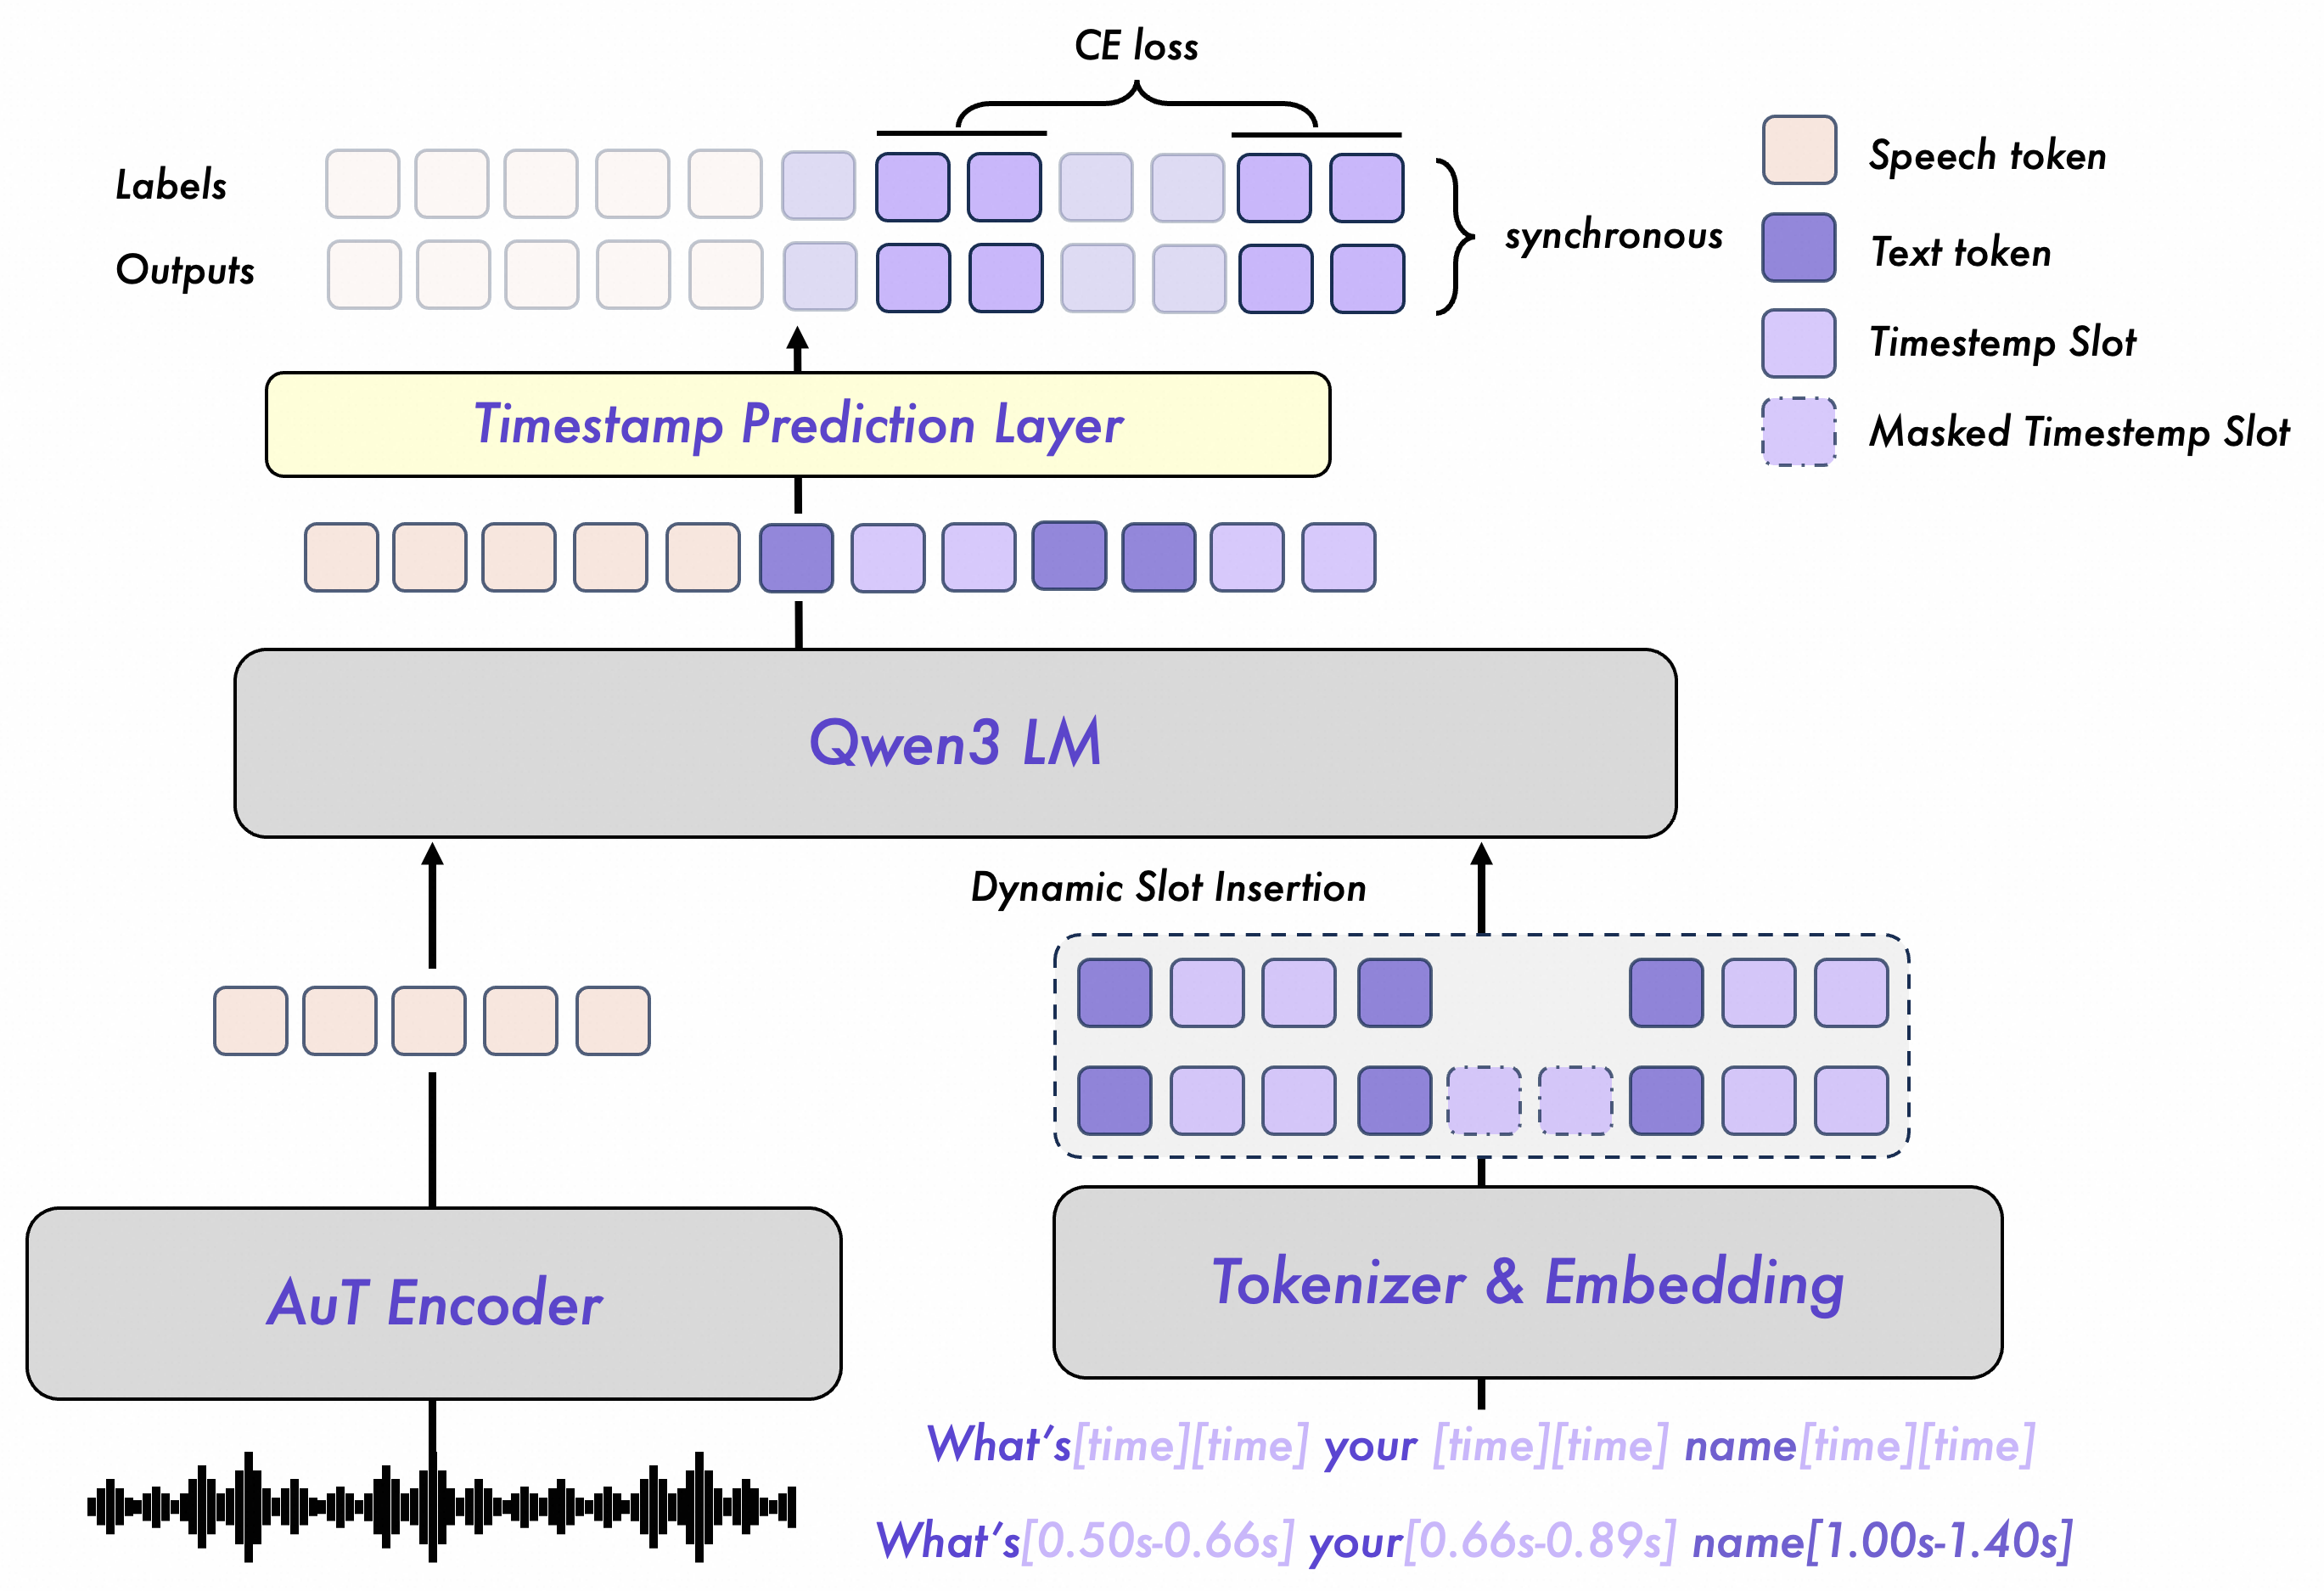
\includegraphics[width=0.7\linewidth]{figures/qwen3asr_fa.png}
    \caption{Illustration of Qwen3-ForcedAligner-0.6B. During training, randomly masked timestamp slots are dynamically inserted into the token sequence to represent word or character boundaries. The combined sequence is fed into Qwen3-0.6B LLM, and a timestamp prediction layer predicts the corresponding timestamp indices for each slot. Supervision is applied with cross‑entropy loss on synchronously aligned label and output sequences.}
    \label{fig:fig2}
\end{figure}

As shown in Figure~\ref{fig:fig2}, Qwen3-ForcedAligner-0.6B employs a pretrained AuT encoder to process the input speech signal and obtain speech embeddings.
The transcript is reformatted by appending start and end timestamp labels to each word or character, after which each timestamp label is replaced with a special token \textit{[time]} and fed into the tokenizer.
Moreover, the timestamp labels in the transcript are discretized into indices by dividing each timestamp value by the 80ms frame duration of the AuT encoder output.
Speech and text embedding sequences are processed by the Qwen3-0.6B LLM, followed by a timestamp prediction linear layer that predicts timestamp indices for the entire input sequence. In this work, the maximum number of classes is 3,750, corresponding to support for speech inputs of up to 300s.

The AuT encoder and the multilingual Qwen3-0.6B LLM jointly provide Qwen3-ForcedAligner-0.6B with multilingual and cross-lingual capabilities. Specifically, the AuT encoder, pretrained on a large-scale multilingual corpus, generates effective frame-level speech embeddings for multiple languages, while the multilingual Qwen3-0.6B LLM handles semantic information across different languages. In addition, the special token \textit{[time]} and the timestamp prediction layer do not rely on language-specific phoneme sets or dictionaries. Details can be found in~\cite{llmfa}.
\subsection{Training Strategies}
Training Qwen3-ForcedAligner-0.6B requires word-level or character-level timestamp labels for a large number of speech–transcript pairs. However, because manual annotation is prohibitively expensive, we use pseudo-timestamp labels generated by the Montreal forced aligner (MFA)~\cite{mfa}, which is among the most accurate existing forced alignment methods. It is important to note that MFA pseudo-labels inherently contain noise and systematic shifts. Qwen3‑ForcedAligner does not simply replicate MFA outputs; instead, it distills and smooths these pseudo-labels, resulting in more stable timestamp predictions with reduced shift.

LALMs typically use a training scheme in which the last token of the output sequence and the first token of the label sequence are removed, creating a one-position offset between the two sequences; the cross-entropy loss is then computed to implement the standard next-token prediction paradigm. However, this paradigm is not suitable for filling timestamp slots. Qwen3-ForcedAligner-0.6B employs causal training, keeping the output and label sequences non-shifted, which allows the model to explicitly recognize timestamp slots during training and predict the timestamp indices to fill them. Moreover, causal training enables Qwen3-ForcedAligner-0.6B to incorporate prior contextual information when predicting the timestamp for the current slot, ensuring global consistency in timestamp prediction.
The cross-entropy loss is computed only in the timestamp slots, thereby focusing the training objective of Qwen3-ForcedAligner-0.6B on timestamp slot filling.

In addition, Qwen3-ForcedAligner-0.6B employs a dynamic slot insertion strategy during training to enhance its generalization capability. Specifically, for each word or character in a sample, the model randomly determines whether to insert start and end timestamp slots afterward.
\subsection{Inference and Usability}
Since the token sequences remain non-shifted during training, users can insert start and end timestamp slots after any word or character, and Qwen3-ForcedAligner-0.6B uses non-autoregressive~(NAR) decoding to predict the timestamp indices for all slots in the transcript simultaneously. Once the timestamp indices are obtained, multiplying each index by 80ms recovers the actual predicted timestamps.

The speed benchmark for Qwen3-ForcedAligner is conducted with FlashAttention and bfloat16. Since the model is non-autoregressive, the inference speed difference between Transformers and vLLM is relatively small; therefore, all our benchmarks are run with Transformers. The results in~\Cref{tab:efficiency_all} show that the model can maintain an RTF close to 0.001 even under high concurrency, i.e., it can process 1,000 seconds of audio per second.

